\graphicspath{{06-Tracker/Figures/}}

\section{Tracker}
\label{Sect:Tracker}

\subsection{Introduction}
\label{SubSect:Tracker_Intro}
% Paul Kyberd reviewed this

The emittance measurement in MICE is performed by two scintillating fibre trackers, placed upstream and downstream of the cooling channel, which will allow for the change in emittance across the cooling channel to be measured.

The trackers are positioned within the bore of superconducting solenoids used to induce helical motion in the incoming particles, from which position and momentum of the particles can be reconstructed and measured.
Each tracker is formed by five stations placed at non-equal intervals to minimized the possible degeneracy in the position measurement~Fig.~\ref{fig:TKR}~(left).
Each station is composed of three planes of doped scintillating fibre of diameter 350~$\mu$, each orientated at 120$^\circ$. The fibres are arranged in doublets as in~Fig.~\ref{fig:TKR}~(right). Scintillation light produced by ionization radiation is readout by visible light photo counters~\cite{ELLIS2011136}.

\begin{figure}
  \begin{center}
    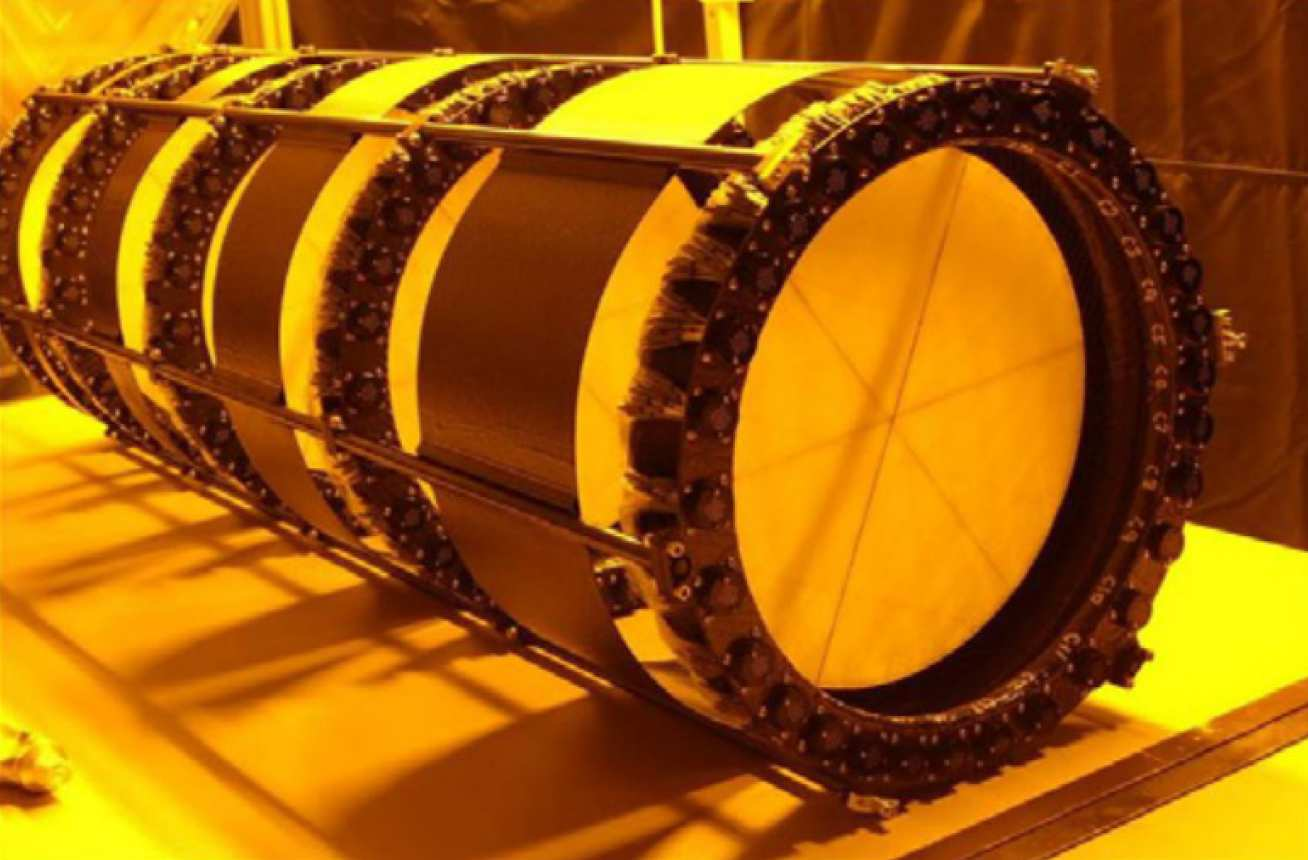
\includegraphics[width=0.49\columnwidth]{./06-Tracker/Figures/TKR1.jpg}
    \hfill
    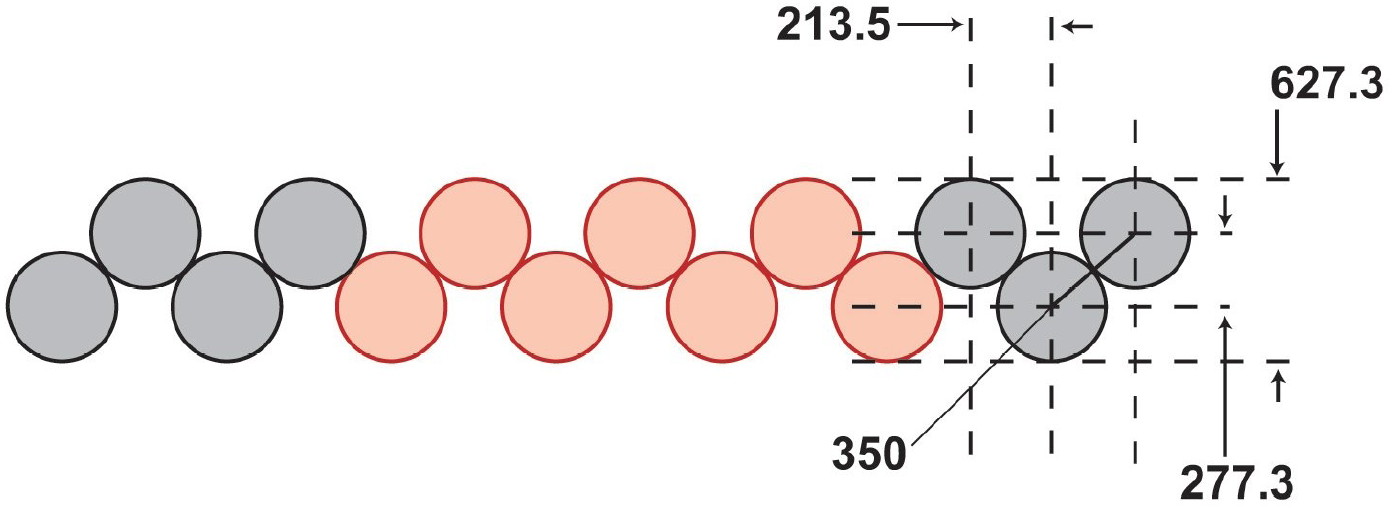
\includegraphics[width=0.49\columnwidth]{./06-Tracker/Figures/TKR2.png}
    \caption{Photograph of one tracker showing the five stations (left) and cross-section of a tracker plane (right) .}
    \label{fig:TKR}
  \end{center}
\end{figure}

The fibres are grouped into channels (seven fibres per channel).
Regarding the tracker reconstruction, hits in individual channel are combined into cluster formed with the neighbour channel.
Spacepoints in each plane are then formed from either two or three clusters.
Spacepoints are associated with individual tracks using a pattern recognition algorithm before a Kalman filter is applied, accounting scattering and energy loss within the tracker.~\cite{NOTE451}.

\subsection{Performance}
\label{SubSect:Tracker_Performance}

\subsection{Tracker resolution in field}
\label{SubSect:Tracker_Resolution}
